\documentclass[../main.tex]{subfiles}

\begin{document}
\section{Skills}
Each Character has a list of skills on the right side of their Character card which can be used during the game. There are several different types of skills that can be used in different scenarios.

\subsection{Ability}
A unit can use an ability skill by performing the Cast Ability Action.

\begin{figure}[h]
    \centering
    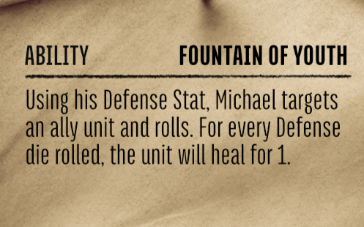
\includegraphics[width=0.75\linewidth]{chapters//Skills/TimeStrikeAbilityGraphic.png}
\end{figure}

\subsection{Passive}
Passive skills are either always in effect, or trigger during described circumstances. Passive skills do not require a unit to perform the Cast Ability Action in order to be used.

\begin{figure}[h]
    \centering
    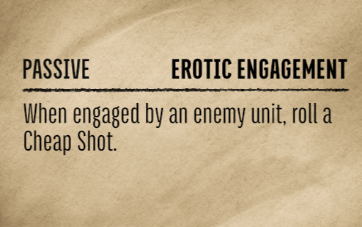
\includegraphics[width=0.75\linewidth]{chapters//Skills/TimeStrikePassiveGraphic.png}
\end{figure}

\subsection{Attack}
Attack skills can be used when a Character performs an attack. 
\begin{figure}[h]
    \centering
    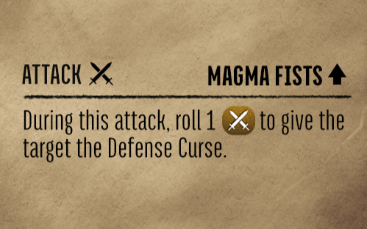
\includegraphics[width=0.75\linewidth]{chapters//Skills/TimeStrikeAttackGraphic.png}
\end{figure}

\textit{Note: Attack skills can rely on Lucky rolls to trigger.}

\subsection{Defense}
Defense skills can be used when a Character defends against an attack.

\begin{figure}[h]
    \centering
    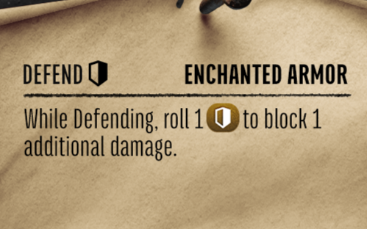
\includegraphics[width=0.5\linewidth]{chapters//Skills/TimeStrikeDefenseGraphic.png}
\end{figure}

\textit{Note: Defense skills can rely on Lucky rolls to trigger.  Notes for all skill types: Skills can alter a unit’s stats when the skill is in effect, so remember to add those when calculating total stat numbers. Skills that require a target will use the Character’s Range stat when targeting unless otherwise stated.}

\section{Luck}
Luck is a mechanic that allows Characters to trigger special effects when rolling Combat Dice. On the Combat Dice you will notice one gold-colored Lucky Attack icon and one gold-colored Lucky Defense icon. Skills or other scenarios may require a certain amount of Lucky Attack or Defense icons to be rolled to trigger different effects or actions.

\begin{figure}[h]
    \centering
    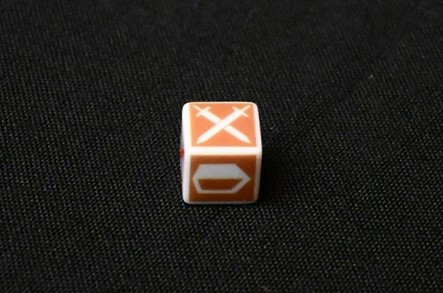
\includegraphics[width=0.5\linewidth]{chapters//Skills/TimeStrikeLuckyAttackIcon.jpg}
\end{figure}
Lucky Attack Icon 

\begin{figure}[h]
    \centering
    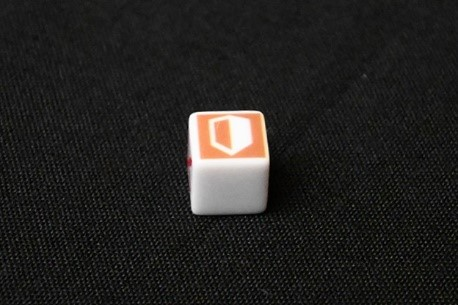
\includegraphics[width=0.5\linewidth]{chapters//Skills/TimeStrikeLuckyDefenseIcon.jpg}
\end{figure}
Lucky Defense Icon

\subsubsection{How to use Luck?}
\begin{enumerate}
    \item When rolling Attack or Defense Combat Dice, check the Character’s skills to see if any have Lucky Attack or Lucky Defense triggers.
    \item If you roll the required number of Lucky Attack or Defense icons, trigger the skill’s effect.
\end{enumerate}

\section{Quests}
Throughout the game, players will be required to draw quests from the quest deck. Quests can be completed by any Character on the team who has the quest. Once a Character completes a quest, they can earn the listed rewards as well as Awaken the Character that completed the quest (Awakening will be covered in the following section). Then discard the quest.

A team can never have more than one quest at a time, so when required to draw a new quest, any previous quests must be discarded.

\section{Awaken}
Characters can Awaken during gameplay which lets them unlock permanent additional stats.

\subsubsection{How to Awaken a Character?}
There are two primary ways to Awaken a Character: completing a quest or defeating an enemy unit. Certain other scenarios, items, or skills can also Awaken Characters.

When a Character Awakens, remove one of the markers to reveal the stat modifiers in the Awakened column. This modifier is unlocked permanently for the rest of the game.

\begin{figure}[h]
    \centering
    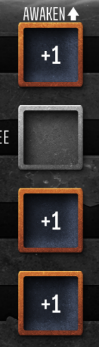
\includegraphics[width=0.25\linewidth]{chapters//Skills/TimeStrikeAwakenGraphic.png}
\end{figure}

\clearpage
\end{document}